
\begin{table}
  \centering \textbf{\textsc{Sobre el autor}} % texto cabecera
  
  \begin{tabular}[t]{crl} % tabla
    \multirow{4}{*}{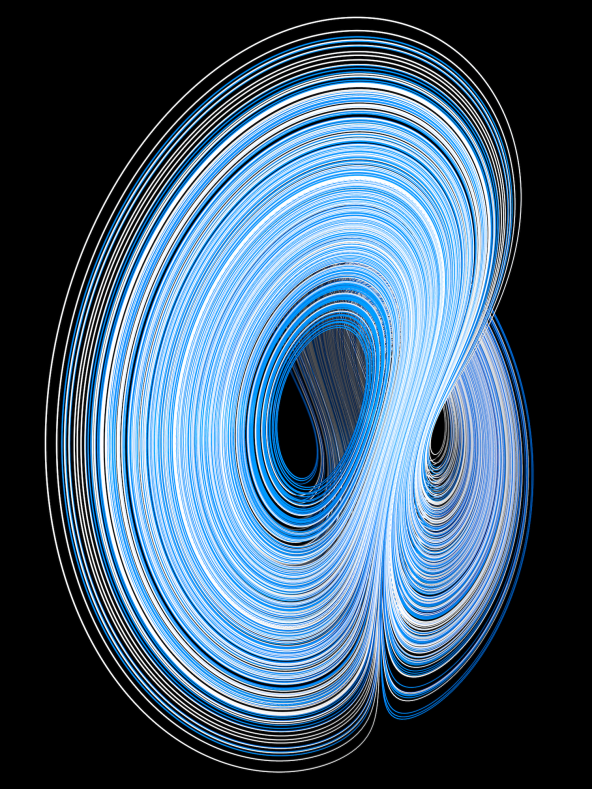
\includegraphics[scale=0.05]{C:/Users/David/Desktop/TFG/TFGLatex/imagenes/lorenz.png}} & \textsf{Nombre} & David Retana Ribeiro \\
                            & \textsf{Titulación} & Grado en Matemáticas \\
                            & \multirow{2}{*}{\textsf{correos}} & \texttt{davidretanaribeiro@gmail.com} \\
                            &                          & \texttt{dr4293@outlook.com} \\
    \textsf{LinkedIn} & \multicolumn{2}{l}{\url{https://www.linkedin.com/in/david-retana-ribeiro-519a56147/}} \\
    \textsf{GitHub}   & \multicolumn{2}{l}{\url{https://github.com/davidRetana}} \\
    \textsf{Kaggle}   & \multicolumn{2}{l}{\url{https://www.kaggle.com/davidretana}} \\
  \end{tabular}
  \label{sobre_el_autor} % etiqueta
\end{table}

\vspace*{1cm}

\noindent \textbf{Convenciones en la escritura del documento}:
\begin{itemize}
  \item Se usará \textit{letra en cursiva} para designar aquellos términos en inglés que no son 
        traducidos al español, como por ejemplo \textit{machine learning}, \textit{cluster}...\\
        También se usará para designar nombres propios como \textit{Creative Commons} o \textit{Apache}.
  \item La letra en \textbf{negrita} quedará reservada para hacer hincapié en ciertos términos que 
        quieran ser remarcados bien sea porque son importantes para el desarrollo del capítulo 
        o porque en ellos se base la idea a explicar en el capítulo.
  \item Las notas al pie de página se usan para explicar conceptos de manera breve y concisa, 
        así como evitar confusiones en la utilización de términos ambiguos.
  \item En numerosas ocasiones aparecerá ejemplos de códigos fuente y comandos de \textit{shell}, 
        éstos aparecerán destacados en un recuadro. Para los comandos \textit{UNIX}, los argumentos encerrados 
        entre signos de desigualdad (< >) indicarán parámetros a completar por el usuario mientras que 
        si están encerrados por corchetes ([ ]) indica que son opcionales.
  \item El código fuente escrito en \textit{Python} seguirá el estilo de marcado por 
        \href{https://www.python.org/dev/peps/pep-0008/}{PEP8}.
  \item En el \autoref{chap:implementacion_paralela}, se utiliza un lenguaje matemático para describir 
        con precisión el modelo de algunos algoritmos que utilizamos. Al comienzo de dicho capítulo 
        se explica en detalle la notación utilizada.
  \item Los enlaces a paginas web son marcados en color \textcolor{blue!80!black}{azul}, mientras que 
        las referencias a puntos de este documento están marcadas de color %\textcolor{violet!50!black}{violeta}.
        \textcolor{Brown}{marrón}.
\end{itemize}

\vspace*{0.5cm}

\noindent Se asume que el lector de este documento tiene una base en matemáticas y estadística así como en algún 
lenguaje de programación, especialmente \textit{Python}. También es recomendable que el lector este
familiarizado con entornos \textit{UNIX} y tenga conocimientos básicos del uso de la terminal.
Este documento no esta enfocado a explicar el funcionamiento de los algoritmos de \textit{machine learning} 
de los que se habla, si no que se centra en desarrollar técnicas que permitan programar estos algoritmos en 
entornos distribuidos de computación.
\newline

\vfill
\begin{flushright}
Este documento ha sido escrito en \LaTeX , usando Texmaker $4.5$ \\
(compiled with Qt $5.2.1$ and Poppler $0.26.5$).\\
Las imágenes han sido realizadas con \url{https://www.draw.io/}.\\
El código fuente se encuentra disponible en mi página de \href{https://github.com/davidRetana/TFGLaTeX}{GitHub}.
\end{flushright}

\clearpage
